\chapter*{Answers to Selected Odd-Numbered Problems}
\addcontentsline{toc}{chapter}{\numberline{}Answers to Selected Odd-Numbered Problems}


\small

{\bf Chapter~\ref{chap:prelim}: Preliminaries}

\Start{S:1.1}: Vectors and Matrices

\exer{c1.1.1A} $(3,2,2)$
\exer{c1.1.1C} $(1,-1,9)$
\exer{c1.1.3a} $(5,0)$
\exer{c1.1.3c} not possible
\exer{c1.1.3e} not possible
\exer{c1.1.4B} $\mattwo{4}{-4}{-11}{11}$


\Start{S:1.2}: \Matlab

\exer{c1.2.1}
(a) $11$;
(b) $\left(\begin{array}{r} 15\\ 3 \\24\end{array} \right)$;
(c) $(-6,-2,-6,-4)$;
(d) $\left(\begin{array}{r} 15 \\ 0 \\ 18 \end{array} \right)$

\exer{c1.2.3a}  $(23.1640, -3.5620, -12.8215)$
\exer{c1.2.4a}  $\left(\begin{array}{rrr} 
-14.0300 & -5.8470 &    7.0600 \\
 -9.7600 & 11.0570 &   -9.6600\end{array}\right)$

\Start{S:1.3}: Special Kinds of Matrices

\exer{c1.1.01a} symmetric
\exer{c1.1.01c} symmetric
\exer{c1.1.01e} symmetric
\exer{c1.1.02b} strictly upper triangular
\exer{c1.1.02d} not upper triangular
\exer{c1.3.1a} $3$
\exer{c1.3.2} $mn$
\exer{c1.3.3b} $\frac{n(n + 1)}{2}$
\exer{c1.3.4a} true
\exer{c1.3.4c} false
\exer{c1.3.5b} \ans $A^t = (3)$

\Start{S:1.4}: The Geometry of Vector Operations

\exer{c1.4.8a} \ans $||x|| = 3$
\exer{c1.4.8c} \ans $||x||=\sqrt{3}$
\exer{c1.4.1a} \ans perpendicular
\exer{c1.4.1bb} \ans not perpendicular
\exer{c1.4.2} $a = \frac{10}{3}$
\exer{c1.4.9a} \ans $x \cdot y = 4$; $\cos\theta =\frac{2}{\sqrt{5}}$
\exer{c1.4.9c} \ans $x \cdot y = 13$; $\cos\theta=\frac{13}{6\sqrt{5}}$
\exer{c1.4.9e} \ans $x \cdot y = 31$; $\cos\theta=\frac{31}{\sqrt{1410}} 
\approx 0.8256$

\vspace{0.08in}
{\bf Chapter~\ref{lineq}: Solving Linear Equations}

\Start{S:2.1}: Systems of Linear Equations and Matrices

\exer{c2.1.8a} \ans $(x,y) = (2,4)$
\exer{c2.1.8c} \ans $(x,y) = (-4,1)$
\exer{c2.1.9}
\ans (a) has an infinite number of solutions; (b) has no solutions.
\exer{c2.1.11}
(a) \ans $p(x) = -x^2 + 5x + 1$
\exer{c2.1.4} \ans 
\begin{verbatim}
ans =
  -12.0495
   -0.8889
    7.8384
\end{verbatim}


\Start{S:2.2} The Geometry of Low-Dimensional Solutions

\exer{c2.2.5} \ans $2x + 3y + z = -5$
\exer{c2.2.7} \ans $z = x$
\exer{c2.2.9}
(a) $u = (2,2,1)$
(b) $v = (1,1,2)$
(c) $\cos\theta = \frac{2}{\sqrt{6}}$; $\theta = 35.2644^\circ$.
\exer{c2.2.1} \ans $(x,y) \approx (2.15,-1.54)$
\exer{c2.2.3} \ans $(x,y,z) = (1,3,-1)$
\exer{c2.2.a5} \ans The function has three relative maxima.


\Start{S:Gauss}: Gaussian Elimination

\exer{c2.3.6a} not in reduced echelon form
\exer{c2.3.6c} not in reduced echelon form
\exer{c2.3.7b} The $1^{st}$, $3^{rd}$, and $5^{th}$ columns contain pivots. 
The system is inconsistent; no solutions.
\exer{c2.3.10a} inconsistent; no solutions
\exer{c2.3.11a} \ans (a) Infinitely many solutions; (b) one variable 
can be assigned arbitrary values.
\exer{c2.3.11c} \ans unique solution
\exer{c2.3.12a} \ans linear
\exer{c2.3.12c} \ans not linear
\exer{c2.3.12e} \ans not linear
\exer{c2.3.1b}  \ans consistent

\exer{c2.3.2} \ans The row echelon form is:
\begin{verbatim}
A = 
       0   1.0000   2.0000   1.0000  14.0000  21.0000        0  -1.0000
       0        0        0   1.0000   3.0000   5.0000        0   9.0000
       0        0        0        0   1.0000  -0.5000        0  -4.7143
       0        0        0        0        0   1.0000        0   0.3457
       0        0        0        0        0        0        0   1.0000
       0        0        0        0        0        0        0        0
\end{verbatim}


\Start{S:2.4} Reduction to Echelon Form

\exer{c2.4.1}
The reduced echelon form of the matrix $A$ is
$\left(\begin{array}{rrrr} 1 & 2 & 0 & 4 \\ 0 & 0 & 1 & 2 \\ 0 & 0 & 0
& 0\end{array}\right)$; $\rank(A)=2$. 

\exer{c2.4.2} \ans four 
\exer{c2.4.3a} \ans consistent; three parameters
\exer{c2.4.3c} \ans inconsistent
\exer{c2.4.4a} \ans $1$
\exer{c2.4.4c} \ans $2$

\Start{S:specialcoeff} Linear Equations with Special Coefficients

\exer{c2.5.1}
$\left(\begin{array}{c} x_1 \\ x_2\end{array}\right) =
\left(\begin{array}{r} \frac{3}{2} - \frac{1}{2}i \\ -\frac{1}{2} -
\frac{1}{2}i\end{array}\right)$
\exer{c2.5.1B}
$\left(\begin{array}{c} x_1 \\ x_2\end{array}\right) =
\left(\begin{array}{r} \frac{1}{2} \\ -\frac{1}{2} \end{array}\right)$
\exer{c2.5.2b}
\begin{verbatim}
A\b =
    0.3006+ 0.2462i
   -0.6116+ 0.0751i
\end{verbatim}


\vspace{0.08in}
{\bf Chapter~\ref{chap:matrices}: Matrices and Linearity}

\Start{S:4.1}: Matrix Multiplication of Vectors

\exer{c4.1.1}  $\vectwo{4}{-11}$
\exer{c4.1.a3a} $\vectwo{6}{-10}$
\exer{c4.1.a3c} $\left(13\right)$
\exer{c4.1.4}
$\left(\begin{array}{rrr} 2 & 3 & -2 \\ 6 & 0 & -5\end{array}\right) 
\left(\begin{array}{r} x_1 \\ x_2 \\ x_3\end{array}\right) = 
\left(\begin{array}{r} 4 \\ 1\end{array}\right)$
\exer{c4.1.7} 
\ans $A = \mattwo{3}{1}{-5}{4}$
\exer{c4.1.9}
\ans No upper triangular matrix satisfies \Ref{eq:avect}, but any 
symmetric matrix of the form $\mattwoc{1}{2}{2}{a_{22}}$ 
satisfies \Ref{eq:avect}.
\exer{c4.1.a10b} 
\begin{verbatim}
b =
  103.5000
  175.8000
 -296.9000
 -450.1000
  197.4000
  656.6000
  412.4000
\end{verbatim}

\exer{c4.1.11} 
\begin{verbatim}
A\b =
   -2.3828
   -1.0682
    0.1794
\end{verbatim}


\Start{s:4.2}: Matrix Mappings

\exer{c4.2.a1a} \ans $(x_1,0)^t$
\exer{c4.2.a1c} \ans $(x_1,3x_1)^t$
\exer{c4.2.1b} \ans $R_{(-45^\circ)}  =
\mattwo{\frac{1}{\sqrt{2}}}{\frac{1}{\sqrt{2}}}{-\frac{1}{\sqrt{2}}}
{\frac{1}{\sqrt{2}}}$
\exer{c4.2.2a} \ans $\mattwo{1}{0}{0}{-1}$
\exer{c4.2.2c} \ans $\mattwo{0}{1}{1}{0}$
\exer{c7.8.2} \ans  $R_{90^\circ} = \mattwo{0}{-1}{1}{0}$
\exer{c4.2.a4a} $A$ maps $x = (1,1)^t$ to twice its length and 
$x = s(0,1)^t$ to half its length.
\exer{c4.2.a4c} $C$ maps $x = (1,0)$ to twice its length and 
$x = (1,2)$ to $-\frac{1}{2}$ times its length.
\exer{c4.2.bb} \ans Matrix $B$ rotates the plane by $\theta =
\approx 3.0585$ counterclockwise and dilatates it by a factor of
$c = \sqrt{5.8} \approx 2.4083$.
\exer{c4.2.4a} $A$ rotates the plane $30^\circ$ clockwise.
\exer{c4.2.4c} $C$ reflects the plane across the line $y = x$.
\exer{c4.2.4e} $E$ maps $(x,y)$ to a point on the line $y = x$; that
point is $(\frac{x + y}{2}, \frac{x + y}{2})$.


\Start{S:linearity}: Linearity


\exer{c4.3.1}
(a) $(-5,11)$;
(b) $(6,8,-16)$;
(c) $(21,7,-10,-2)$
\exer{c4.3.3}  $\alpha = -\frac{7}{5}$; $\beta = -\frac{3}{5}$
\exer{c4.3.5} \ans $\alpha = \frac{5}{13}\gamma + \frac{7}{13}$ and 
$\beta = -\frac{14}{13}\gamma - \frac{4}{13}$
\exer{c4.3.6b} \ans not linear
\exer{c4.3.6d} \ans not linear
\exer{c4.3.8} \ans  $A = \matthree{0}{-1}{-1}{1}{0}{2}{1}{-2}{0}$
\exer{c4.3.10} \ans $A = \matthree{0}{1}{0}{0}{0}{1}{1}{0}{0}$
\exer{c4.3.14}  The mapping rotates a 2-vector $90^\circ$ clockwise and 
then it halves its length.


\Start{S:Superposition}: The Principle of Superposition

\exer{c4.4.1}
(a) \ans $v_1 = \vecthree{-1}{1}{0}; v_2 = \vecthree{-1}{0}{1}$
(b) \ans $w_1 = \vecthree{1}{0}{-1}; w_2 = \vecthree{0}{1}{-1}$

\exer{c4.4.3}
(a) \ans $s\vecthree{-11}{7}{1}$;
(b) \ans $\vecthree{1}{1}{1}$;
(c) \ans $\vecthree{1}{1}{1} + s\vecthree{-11}{7}{1}$



\Start{S:4.6}: Composition and Multiplication of Matrices

\exer{c4.6.-1a} $AB=\mattwo{-2}{0}{7}{-1}$; $BA= \mattwo{-2}{0}{5}{-1}$
\exer{c4.6.-1c} Neither $AB$ nor $BA$ is defined. 
\exer{c4.6.0a}  $\mattwo{-11}{8}{-3}{2}$
\exer{c4.6.0c} $\matthree{-4}{13}{3}{-12}{11}{-11}{3}{-1}{4}$
\exer{c4.6.1} \ans $B=\mattwo{b_{11}}{0}{0}{b_{22}}$
\exer{c4.6.3} $\matthree{10}{-5}{15}{-5}{6}{-4}{15}{-4}{26}$
\exer{c4.7.1b} Neither $AB$ nor $BA$ is defined.



\Start{S:4.7}: Properties of Matrix Multiplication

\exer{c4.7.4}
$B = \matthree{1}{1}{\frac{1}{2}}{0}{1}{1}{0}{0}{1}$; 
$C = \cmatthree{1}{t}{\frac{t^2}{2}}{0}{1}{t}{0}{0}{1}$


\Start{S:SLS}: Solving Linear Systems and Inverses


\exer{c4.8.3} \ans $a \neq 0$ and $b \neq 0$
\exer{c4.9.3a} \ans
$A^{-1} = \dps\frac{1}{10}\matthree{-8}{32}{-9}{2}{2}{1}{2}{-8}{1}$
\exer{c4.9.6}
\ans  $A$ is invertible for any $a$, $b$, and $c$, and
$A^{-1} = \left(\begin{array}{rrc} 1 & -a & -b + ac \\ 0 & 1 & -c 
\\ 0 & 0 & 1 \end{array}\right)$.

\exer{c4.9.7b}
Type {\tt N = [B eye(4)]} in \Matlab and then row reduce {\tt N} to obtain
\begin{verbatim}
ans =
1.0000        0        0        0   -1.5714   -0.4286         0    1.4286
     0   1.0000        0        0    0.7429    0.0571    0.2000   -0.4571
     0        0   1.0000        0   -0.9143    0.3143   -0.4000    0.4857
     0        0        0   1.0000   -0.6000   -0.2000   -0.2000    0.6000
\end{verbatim}


\Start{S:det2x2}: Determinants of $2\times 2$ Matrices

\exer{c4.9.1}  $\mattwo{2}{-1}{-3}{2}$
\exer{c7.8.4C} \ans  $y=\frac{29}{11}$
\exer{c3.8.AA} \ans $A$ is invertible; $\det(A) = 4$.
\exer{c3.8.AC} \ans $A$ is not invertible; $\det(A) = 0$


\vspace{0.08in}
{\bf Chapter~\ref{chap:SolveOdes}: Solving Ordinary Differential Equations}


\Start{S:growthmodels}: A Single Differential Equation

\exer{c3.1.a01a}
\ans $\dps x(t) = \frac{5 - \cos(2t)}{2}$
\exer{c3.1.a01c} $\dps x(t) = 2 - \frac{1}{t}$
\exer{c3.1.bb}
\ans $x_1(t)$ is a solution; $x_2(t)$ is not a solution.
\exer{c3.1.bd}
\ans $x_1(t)$ is not a solution; $x_2(t)$ is a solution.
\exer{c3.1.2}
\ans $t_1 = -\frac{1}{3} \ln(0.5)$
\exer{c3.1.4}
\ans $P_{instant}(1.5) = \mbox{\$}11\mbox{,}190.72$;
$P_{monthly}(1.5) = \mbox{\$}11\mbox{,}186.81$
\exer{c3.1.6}
\ans If the population doubles every $50$ years, then
$r = \frac{1}{50}(\ln 2)$.  If the population doubles every $25$
years, then $r = \frac{1}{25}(\ln 2)$.
\exer{c3.1.7} \ans Snow started falling at 11:23 am.
\exer{c3.1.a78b}  The graph is shown on the left in the figure.
\exer{c3.1.a78d}  The graph is shown on the right in the figure.
\begin{figure}[ht]
                       \centerline{%
                       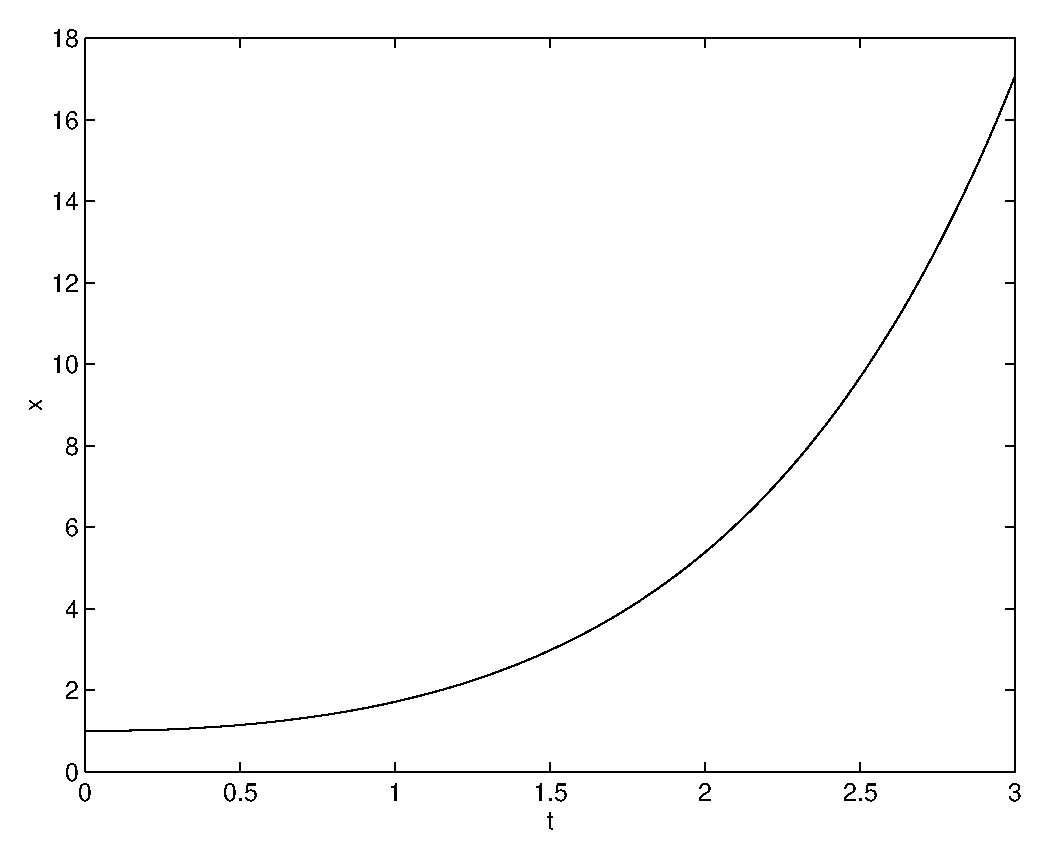
\psfig{file=exfigure/3-1-a78b.eps,width=1.35in}
                       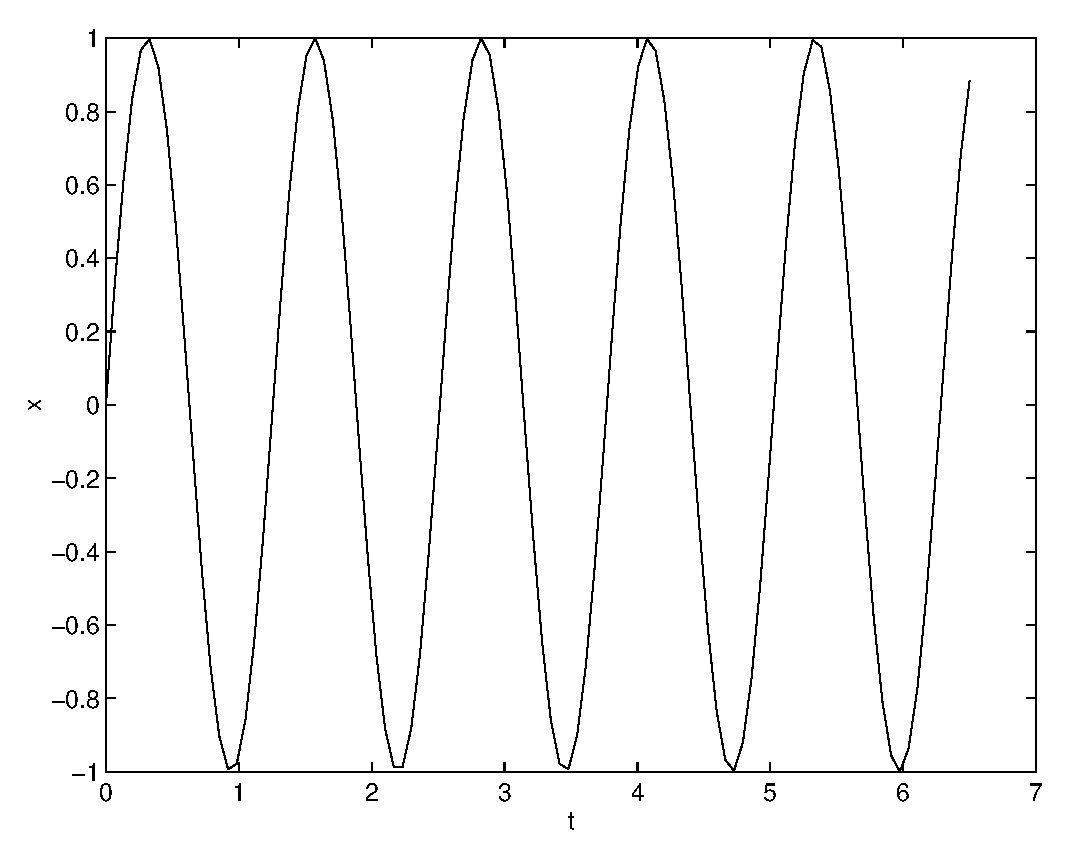
\psfig{file=exfigure/3-1-a78d.eps,width=1.35in}}
\end{figure}

\exer{c3.1.9}
\ans After two years Statewide returns more interest than Intrastate.  
After one year, Intrastate returns more.


\Start{S:3.2}: Graphing Solutions to Differential Equations

\exer{c3.2.1A} increasing
\exer{c3.2.1C} increasing
\exer{c3.2.3A} nonautonomous
\exer{c3.2.3C} autonomous
\exer{c3.2.2}  The minimum value is $\approx -1.39$.  

%\exer{exer:at}  Computer experiment.

\Start{S:PSP&E}: Phase Space Pictures and Equilibria

\exer{c3.3.1} \ans $0.055 \leq x(0) \leq 0.109$
\exer{c3.3.3} \ans $\lambda > 0$
\exer{c3.3.6B}
\ans $x=4$ and $x = -2$ are unstable equilibria, and $x = 0$ is stable.
\exer{c3.3.6D} \ans $x = -3+2\sqrt{2}$ is an unstable equilibrium and 
$x = -3-2\sqrt{2}$ is stable.
\exer{c3.3.10a} \ans autonomous
\exer{c3.3.10c} nonautonomous



\Start{sec:sov}: Separation of Variables

\exer{c14.1.1a} \ans Separation of variables can be used; set $g(x) = x^{1/2}$ 
and $h(t) = \cos t$.
\exer{c14.1.1c} \ans Separation of variables cannot be used.
\exer{c14.1.5a} \ans $x(t) = -e^{-3t}$
\exer{c14.1.5c} \ans $x(t) = \frac{1}{9}(2t^{3/2} + 1)^2$
\exer{c14.1.8b} \ans $x(t) = Ke^{5t} - \frac{2}{5}$ for some $K \geq 0$.  
$x(t) = x_0 = -\frac{2}{5}$ is a constant solution.


\Start{sec:UncoupledLS}: Uncoupled Linear Systems of Two Equations

\exer{c3.5.1A} \ans $(0,0)$ and $(1,1)$
\exer{E:uncoupleda} \ans The origin is a saddle.
\exer{E:uncoupledc} The origin is not a saddle, a source or a sink. 
\exer{c3.4.5}  \ans Trajectories approach the origin tangent to the $y$-axis 
if $A < D < 0$. 
\exer{c3.4.7} \ans Identical initial conditions have identical trajectories
for the two systems. 


\Start{s:3.5}:  Coupled Linear Systems

\exer{c3.5.a01}
(a) Trajectories converge to the origin when $D < 0$;
(b) trajectories move away from the origin when $D > 0$;
(c) trajectories form circles around the origin when $D = 0$.
\exer{c3.5.5a} \ans Both function pairs are solutions.
\exer{c3.5.5c} \ans $(e^t\sin{t},e^t\cos{t})$ is a
solution, whereas $(3e^t,-2e^t)$ is not.


\Start{S:IVP&E}:  The Initial Value Problem and Eigenvectors

\exer{c4.1.5}
$\dps\frac{dX}{dt} = \mattwo{4}{5}{2}{-3}X$ where $X(t)=(x_1(t),x_2(t))^t$.
\exer{c4.5.3} \ans $(1,1)^t$ is an eigenvector of $C$ with eigenvalue $a + b$; 
$(1,-1)^t$ is an eigenvector with eigenvalue $a - b$.
\exer{c4.5.5a} $(-1,2)^t$ is an eigenvector of $B$ with eigenvalue $6$, and 
$(-2,1)^t$ is an eigenvector with eigenvalue $3$.
\exer{c4.4.5} (a) \ans $\alpha = 1$; $\beta = 1$ 


\Start{S:evchp}:  Eigenvalues of $2\times 2$ Matrices

\exer{c4.9.2}
\ans $\lambda = 5$ or $\lambda = -1$
\exer{c6.4.1b} The determinant is $23$, the trace is $7$, and
the characteristic polynomial is $\lambda^2-7\lambda+23$.
\exer{c6.4.1d} The determinant is $0$, the trace is $9$, and
the characteristic polynomial is $\lambda^2-9\lambda$.
\exer{c6.4.2b} \ans The eigenvalues are $\frac{-3 + \sqrt{17}}{2}$ and 
$\frac{-3 - \sqrt{17}}{2}$.
\exer{c7.8.6a} The eigenvectors are $(2,1)^t$ with eigenvalue
$4$, and $(1,-1)^t$ with eigenvalue $-2$.
\exer{c7.8.7} \ans  $\lambda \approx 2.5291 \pm 2.1111i$.



\Start{S:IVPR}: Initial Value Problems Revisited

\exer{c4.10A.1a} \ans $X(t) = 4e^{2t}\vectwo{1}{1} - 3e^t\vectwo{1}{0}$
\exer{c4.10A.1c} \ans $X(t) = \frac{8}{3}e^t\vectwo{1}{2} - 
\frac{5}{3}e^{-2t}\vectwo{2}{1}$
\exer{c4.10A.2} \ans $X(t) = \frac{1}{5}e^{-t}\vectwo{1}{2} + 
\frac{2}{5}e^{4t}\vectwo{2}{-1}$
\exer{c4.10A.3b} \ans $X(t) \approx 1.0860e^{-1.8035t}\vectwo{-0.9005}{ 0.4348}
- 2.4527e^{4.4835t}\vectwo{-0.8880}{-0.4598}$
\exer{c4.10A.4b} \ans $X(0.5) = (1.621,0.291)^t$; the two methods agree to 
three decimal places.


\Start{S:TransitionApplied}: Markov Chains

\exer{c4.10.2b} The matrix $Q$ is not a Markov matrix, since there is no
positive integer $k$ for which the $2$nd, $1$st column of $Q^k > 0$.
\exer{c4.10.3} 
$\left(\begin{array}{rrrrr}
\frac{1}{3} & 0 & \frac{1}{3} & \frac{1}{3} & 0 \\
\frac{1}{3} & \frac{1}{3} & \frac{1}{3} & 0 & 0 \\
0 & 0 & \frac{1}{2} & \frac{1}{2} & 0 \\
0 & 0 & 0 & \frac{1}{2} & \frac{1}{2} \\
\frac{1}{4} & \frac{1}{4} & 0 & \frac{1}{4} & \frac{1}{4}
\end{array}\right)$
\exer{c4.10.5}
(a) \ans  ${\tt PDOG} = 
\left(\begin{array}{rrrr} 0 & \frac{1}{3} & \frac{1}{3} &
\frac{1}{3} \\ 1 & 0 & 0 & 0 \\ 0 & 0 & 0 & 1 \\
0 & \frac{1}{2} & \frac{1}{2} & 0 \end{array}\right)$.
(b) $\frac{7}{36}$;
(c) \ans  $0$;
(d) \ans After a large number of steps, there will be approximately $23$
dogs in each of rooms 1, 2, and 3, and $31$ dogs in room 4.
\exer{c4.10.7}
(a) $11.62\%$
(b) $14.07\%$
(c) $(P^t)^4\left(\begin{array}{r} 20 \\ 20 \\ 20 \\ 20 \\ 20
\end{array}\right) = \left(\begin{array}{r} 14.1466 \\ 22.1620 \\
21.2874 \\ 30.0624 \\ 12.3417 \end{array}\right)$
(d) \ans An eigenvector of $P^t$ with eigenvalue 1 is
$V = \left(\begin{array}{r} 0.1408 \\ 0.2195 \\ 0.2154 \\ 0.3032
\\ 0.1211 \end{array}\right)$.
\exer{c4.10.9}
\ans $1.53\%$.

\vspace{0.08in}
{\bf Chapter~\ref{C:vectorspaces}: Vector Spaces}

\Start{S:5.1}: Vector Spaces and Subspaces

\exer{c5.1.3} $V_1$ and $V_3$ are identical.
\exer{c5.1.4b} \ans not a subspace
\exer{c5.1.4c} subspace
\exer{c5.1.4e} subspace
\exer{c5.1.5a} \ans not a subspace
\exer{c5.1.5c} \ans subspace
\exer{c5.1.5e} \ans not a subspace
\exer{c5.1.7a} \ans subspace when $c = 0$; not a subspace when $c \neq 0$ 

\Start{S:5.2}:  Construction of Subspaces

\exer{c5.2.1a} \ans $\Span\{(1,0,-4)^t,(0,1,2)^t\}$
\exer{c5.2.1c}  \ans  $\Span\{(1,0,-1)^t,(0,1,-1)^t\}$

\exer{c5.2.2a} \ans $\Span\{(-2,1,0,0,0)^t,(-1,0,-4,1,0)^t\}$
\exer{c5.2.2c} \ans $\Span\{(-2,-1,1)^t\}$
\exer{c5.2.3}
\ans $\left(\begin{array}{rrrr} 1 & 1 & 0 & 0 \\ 0 & 0 & 1 & 1
\end{array}\right)$
\exer{c5.2.5} \ans $(2,20,0)^t = -4w_1 + 6w_2$
\exer{c5.2.6b} $t^4\not\in W$
\exer{c5.2.6d} \ans $y(t) = 0.5t^2\in W$, but $\{y(t),x_2(t)\}$ does not 
span $W$.


\Start{S:5.3}:  Spanning Sets and \Matlab


\exer{c5.3.1a}  $\Span\{(0.3225, 0.8931, -0.0992, 0.2977)^t,
(0,-0.1961,0.5883,0.7845)^t\}$

\exer{c5.3.1c} $\Span\{(-0.8452,-0.1690,0.5071)^t\}$.
\exer{c5.3.3} \ans $\Span\{(-1, -3, 1, 0)^t, (3/4, 2, 0, 1)^t\}$
\exer{c5.3.4b} \ans $v_2\not\in W$

\Start{S:5.4}:  Linear Dependence and Linear Independence

\exer{c5.4.3} \ans linearly dependent.
\exer{c5.4.8b} \ans linearly dependent


\Start{S:5.5}:   Dimension and Bases


\exer{c5.5.3}
\ans $\{(1,1,1,0), (-2,-2,0,1)\}$ is a basis; the dimension is two.
\exer{c5.5.5} $\dim {\cal P}_2=3$; $\dim {\cal P}_n = n+1$


\Start{S:5.6}:  The Proof of the Main Theorem

\exer{c5.7.1a} \ans  A plane with $N = n_3(-\frac{3}{2}, 1, 1)$.
\exer{c5.7.1c} \ans A plane with $N = n_3(0,0,1)$.
\exer{c5.6.1}
(a) $5$; (c)  $5 - r$; (d) $5 - r$
\exer{c5.6.4}
(a) \ans $\lambda \neq 2$; (b) $\lambda = 2$
\exer{c5.6.6} \ans $\{(1,0,0,-\frac{1}{2},\frac{3}{2})$, $(0,1,0,\frac{1}{2},
-\frac{1}{2})$, $(0,0,1,\frac{1}{2},\frac{3}{2})\}$ 


\vspace{0.08in}
{\bf Chapter~\ref{Chap:Planar}: Closed Form Solutions for Planar ODEs}

\Start{S:6.1}:  The Initial Value Problem

\exer{c6.1.03a}
\ans The associated eigenvalues are $2$ and $-1$.
\exer{c6.1.03c} $2e^{2t}\vectwo{2}{-3} + e^{-t}\vectwo{-7}{11}$
\exer{c6.1.06a} \ans The associated eigenvectors are $(1,1)^t$ and $(1,-1)^t$.
\exer{c6.1.06c} $4\vectwo{1}{1} - 2e^{2t}\vectwo{1}{-1}$
\exer{c6.1.1c} $(-\sin t,\cos t)$
\exer{c6.1.2a} \ans  $e^{-2t}(1,0)$
\exer{c6.1.3a}
\ans The associated eigenvalues are $-1$, $-2$, and $-3$.

\exer{c6.1.3c} \ans $-2e^{-2t}\vecthree{2}{-1}{2} + e^{-3t}\vecthree{6}{-3}{7}$
\exer{c6.1.4} (b) \ans The eigenvalues are $2$ and $-1$; 
(c) \ans $2e^{2t}\vectwo{1}{-1} + e^{-t}\vectwo{2}{1}$


\Start{S:TDM}: Closed Form Solutions by the Direct Method

\exer{c6.6.1b}
\ans $3\cos^2\theta\sin\theta - \sin^3\theta$

\exer{c6.6.2b}
\ans $X(t) =
\alpha_1\cvectwo{5e^{2t}\cos(3t)}{e^{2t}(2\cos(3t) + \sin(3t))} +
\alpha_2\cvectwo{5e^{2t}\sin(3t)}{e^{2t}(2\sin(3t) - \cos(3t))}$

\exer{c6.6.2d} \ans 
$X(t) = 
\alpha e^{-2t}\cvectwo{2}{1} + \beta e^{-2t}\cvectwo{2t + 1}{t + 1}$


\Start{S:Matrixexp}: Solutions Using Matrix Exponentials


\exer{c6.2.1} \ans $m = 7$
\exer{c6.2.3}
One example is $C_1 = \mattwo{1}{-2}{3}{1} \AND C_2 = \mattwo{-2}{3}{-1}{-2}$.

\exer{c6.2.4b} \ans $e^{tC} =
\cmatthree{1}{t}{\frac{t^2}{2}}{0}{1}{t}{0}{0}{1}$


\Start{S:LNFPS}: Linear Normal Form Planar Systems


\exer{c6.3.1}
\ans  $\vectwo{x(t)}{y(t)} = \vectwo{e^{2t}(\cos(3t) - 2\sin(3t))}
{-e^{2t}(\sin(3t) + 2\cos(2t))}$
\exer{c6.3.25}
\ans $e^{tC} = e^{2t}(I_n + tA + \frac{t^2}{2}A^2)$



\Start{S:6.5}: Similar Matrices

\exer{c6.5.3a}
\ans not similar
\exer{c6.5.6}
\ans $\dps e^A = e^2\mattwo{2}{-1}{1}{0}$


\Start{S:6.6}: Formulas for Matrix Exponentials


\exer{c6.6.2}
\ans $X(t) = -3e^t\vectwo{1}{1} + e^{2t}\vectwo{1}{2}$
\exer{c6.6.4}
\ans $X(t) = e^t\vectwo{2\sin{t} + \cos{t}}{-3\sin{t} + \cos{t}}$


\Start{S:SOE}: Second Order Equations

\exer{c6.7.1}
\ans  $t \approx 1.63$ seconds
\exer{c6.6.hoa}
\ans $x(t) = \alpha e^t + \beta e^{-3t}$
\exer{c6.6.hoc}
\ans $x(t) = e^{-t}(\alpha \cos{t} + \beta \sin{t})$
\exer{c6.6.tfb} \ans false


\vspace{0.08in}
{\bf Chapter~\ref{Chap:PlanarQ}: Qualitative Theory of Planar ODEs}

\Start{S:6.7}: Sinks, Saddles, and Sources

\exer{E:stabmata} \ans not asymptotically stable
\exer{E:stabmatc} \ans not asymptotically stable
\exer{E:sisasob} \ans saddle
\exer{E:sisasod} \ans source
\exer{E:sisasof} \ans source
\exer{E:sssb} \ans saddle
\exer{E:sssd} \ans sink
\exer{E:simb}
(a) \ans $P \approx \mattwo{7.1063}{0}{0}{0.7106}$;
$P$ stretches the $x$-coordinate of a vector and shrinks the $y$-coordinate.
(b) \ans The solutions of $\dot{X} = CX$ are obtained from the solutions
of $\dot{X} = BX$ by stretching the $x$-coordinate by a factor of $7.1063$
and the $y$-coordinate by a factor of $0.7106$.


\Start{S:PlanarSystems}: Phase Portraits of Sinks

\exer{c6.8.1a} \ans saddle
\exer{c6.8.1c} \ans saddle
\exer{c6.8.2b}
\ans A possible matrix is $\mattwo{-0.5}{-1}{1}{-0.5}$.
\exer{c6.8.2d}
\ans A possible matrix is $\mattwo{-1}{0}{1}{-2}$.
\exer{c6.8.4a} (a) no; (b) none


\Start{S:6.9}: Phase Portraits of Nonhyperbolic Systems

\exer{c6.9.1a} \ans One such matrix is $\mattwo{0}{-1}{1}{0}$.
\exer{E:PPb} \ans asymptotically stable for $A$ and unstable
for $B$, $C$, and $D$
\exer{E:PPd} \ans $\det(A)>0$, $\det(D)>0$, $\det(B)<0$, $\det(C)=0$
\exer{E:PQa} \ans  hyperbolic; spiral source
\exer{E:PQc} \ans  hyperbolic; improper nodal source
\exer{E:PQe} \ans  not hyperbolic; center
\exer{E:PQg} \ans hyperbolic; saddle


\vspace{0.08in}
{\bf Chapter~\ref{C:D&E}: Determinants and Eigenvalues}


\Start{S:det}: Determinants

\exer{c10.1.1a} \ans $-28$
\exer{c10.1.1c} \ans $14$
\exer{c10.1.5a} \ans $-4$
\exer{c10.1.6} (a) \ans $1$ and $-1/3$; (b) \ans yes

\exer{c10.1.b7b}
$B_{11} = \matthree{7}{-2}{10}{0}{0}{-1}{4}{2}{-10}$;
$B_{23} = \matthree{0}{2}{5}{0}{0}{-1}{3}{4}{-10}$;
$B_{43} = \matthree{0}{2}{5}{-1}{7}{10}{0}{0}{-1}$


\Start{S:eig}: Eigenvalues

\exer{c10.2.1a}
\ans $p_A(\lambda) = -\lambda^3 + 2\lambda^2 + \lambda - 2$; 
the eigenvalues are $1$, $-1$, and $2$.
\exer{c10.2.2}
\ans $\{(-1,1,0)^t, (1,0,1)^t\}$
\exer{c10.2.4}
(a) \ans The eigenvalues are $3$ and $-2$ with corresponding eigenvectors 
$(1,-1)^t$ and $(1,-2)^t$.
(c) \ans $(2x_1 + x_2, -x_1 - x_2)$. 
\exer{c10.2.7b} false
\exer{c10.2.9a}
(a) The eigenvalues are $-0.5861 \pm 20.2517$, $-12.9416$, $-9.1033$, 
and $5.2171$.  The trace is $-18$.  The characteristic polynomial is
$\lambda^5 + 18\lambda^4 + 433\lambda^3 + 6296\lambda^2 +
429\lambda - 252292$.
\exer{c10.2.10}
\ans $B$ is the zero matrix.


%\Start{A:det}: Appendix: Existence of Determinants

\vspace{0.08in}
{\bf Chapter~\ref{C:LMCC}: Linear Maps and Changes of Coordinates}


\Start{Sect:linmap}: Linear Mappings and Bases

\exer{c7.2.1}
$A = \left(\begin{array}{rrr} -7 & -11 & 3 \\ -4 & -7 & 2
\end{array}\right)$


\Start{S:5.8}: Row Rank Equals Column Rank

\exer{c5.8.1}
\ans The possible choices are $\alpha_3(-1,-1,1)$ and
$\beta_3(-\frac{7}{5},-\frac{9}{5},1)$.

\exer{c5.8.3}
(a) $\{(1,0,1,0), (0,1,-1,0), (0,0,0,1)\}$ is a basis for the row space of 
$A$; the row rank of $A$ is $3$.
(b) The column rank of $A$ is $3$; $\{(1,0,0)$, $(0,1,0)$, $(0,0,1)\}$ is 
a basis for the column space of $A$.
(c) $\{(-1,1,1,0)\}$ is a basis for the null space; the nullity of 
$A$ is $1$.  
(d) The null space is trivial and the nullity of $A^t$ is $0$.


\Start{S:coordinates}: Vectors and Matrices in Coordinates

\exer{c7.1.1} \ans $[v]_{\cal W} = (7,4)$
\exer{c7.1.6} \ans $[v]_W = (-2,2,-1)$
\exer{c7.3.4} \ans $[L]_{\cal W}$ is diagonal in the basis
${\cal W} = \left\{\vectwo{1}{2},\vectwo{2}{3}\right\}$


\Start{MALT}: Matrices of Linear Maps on a Vector Space

\exer{c7.1.2} \ans $C_{\cal WZ} = \mattwo{2}{3}{-1}{-2}$
\exer{c7.5.A}  (a) \ans $A$ fixes $w_1$, moves $w_2$ to $w_3$, and moves 
$w_3$ to $-w_2$.
(b) \ans $[L_A]_{\cal W} = \matthree{1}{0}{0}{0}{0}{-1}{0}{1}{0}$
(c) \ans $[L_A]_{\cal W}$ fixes $e_1$, moves $e_2$ to
$e_3$, and moves $e_3$ to $-e_2$.



\vspace{0.08in}
{\bf Chapter~\ref{Chap:LinTrans}: Orthogonality}

\Start{S:orthonormal}: Orthonormal Bases

\exer{c7.4.1}
\ans  $\frac{1}{\sqrt{3}}(1,1,-1)$ and $\frac{1}{\sqrt{2}}(0,1,1)$

\Start{S:LSA}: Least Squares Approximations

\exer{c7.5.1}
\ans $\frac{1}{5}(3,4)$ and $\frac{1}{5}(-4,3)$


\Start{S:7.6}: Least Squares Fitting of Data

\exer{c7.6.1}
(a) \ans $m \approx 0.4084$ and $b \approx 0.9603$, where $m$ and $b$ are in
billions.
(b) In 1910 $P \approx 1369$ million people.
(c) \ans The prediction for 2000 is likely to be low.
\exer{c7.6.3}
\ans Let $R$ be the number of days in the year with precipitation and
let $s$ be the percentage of sunny hours to daylight hours.  Then the
best linear estimate of the relationship between the two is $R \approx 199.2 -156.6s$. 


\Start{S:symmetric}: Symmetric Matrices

\exer{exer:powita}
\ans The eigenvectors are $(1,1)$ and $(1,-1)$; the eigenvalues are $4$ and 
$-2$; 

\exer{exer:powitc}
\ans The eigenvectors are $(1,1)$ and $(1,-1)$;
the eigenvalues of $C$ are $-2$ and $2.01$.



\Start{S:QR}: Orthogonal Matrices and $QR$ Decompositions

\exer{c7.9.1a} \ans not orthogonal
\exer{c7.9.1c} orthogonal
\exer{c7.9.1e} not orthogonal
\exer{c7.9.3a} $H = \mattwo{0}{-1}{-1}{0}$

\exer{c7.9.3c} 
$H = \frac{1}{27}\matthree{25}{2}{10}{2}{25}{-10}{10}{-10}{-50}$
\exer{c7.9.4}
\ans $\mattwo{-\frac{3}{5}}{\frac{4}{5}}{\frac{4}{5}}{\frac{3}{5}}$
\exer{c7.5.5a} The orthonormal basis generated by the command {\tt [Q R] = qr(A,0)} is:
\begin{verbatim}
v1 =          v2 =
   -0.7071        0.7071
    0.7071        0.7071
\end{verbatim}

\exer{c7.5.5c}
The orthonormal basis generated by the command {\tt [Q R] = qr(A,0)} is:
\begin{verbatim}
v1 =          v2 =          v3 = 
   -0.2673        0.0514       -0.9623
    0.5345       -0.8230       -0.1925
   -0.8018       -0.5658        0.1925
\end{verbatim}

\exer{c7.5.6}
\ans
\begin{verbatim}
H1 =                                   H2 =
   0.6245  -0.7220  -0.2744   0.1155      0.2807   0.6679  -0.3083  -0.6165
  -0.7220  -0.3885  -0.5276   0.2222      0.6679   0.3798   0.2862   0.5725
  -0.2744  -0.5276   0.7995   0.0844     -0.3083   0.2862   0.8679  -0.2642
   0.1155   0.2222   0.0844   0.9645     -0.6165   0.5725  -0.2642   0.4716

H =
   -0.2935    0.1305   -0.6678   -0.6714
   -0.4365   -0.6536   -0.4053    0.4669
   -0.7279   -0.1065    0.6051   -0.3043
   -0.4398    0.7378   -0.1536    0.4885
\end{verbatim}


\vspace{0.08in}
{\bf Chapter~\ref{C:NPS}: Autonomous Planar Nonlinear Systems}

\Start{S:introAPNS}: Introduction

\exer{c8.1.1}
There are three equilibria in the interval $[-3,1]$; $x\approx -2.910$ 
and $x\approx 0.925$ are asymptotically stable 
$x \approx -0.408$ is unstable.
\exer{c8.1.3a} A valid initial condition is $X(0) = (1,4)$. 
\exer{c8.1.3c} A valid initial condition is $X(0) = (1,2)$. 


\Start{S:linearization}: Equilibria and Linearization

\exer{c8.2.1} (b) \ans $\dps\lim_{t \to \infty} x(t) = -\infty$
\exer{c8.2.3}
(b) \ans If there exists a positive equilibrium $p_e$, then
$\dps\lim_{p \to \infty} p(t) = p_e$.  If no positive equilibrium
exists, then $\dps\lim_{p \to \infty} p(t) = \infty$.
\exer{c8.2.4b} \ans spiral source
\exer{c8.2.4d} \ans not hyperbolic
\exer{c8.2.5}
(a) \ans $(1,0)$ and $(0,1)$
(b) \ans $(1,0)$ is a saddle; $(0,1)$ is a spiral sink.
\exer{c8.2.7}
(a) $(0,0)$ and $(\sqrt{2.2},0)$, $(-\sqrt{2.2},0)$;
(c) \ans $(\sqrt{2.2},0)$ is not hyperbolic when $a = -2.1\left/\sqrt{2.2}\right.$; 
$(-\sqrt{2.2},0)$ is not hyperbolic when $a = 2.1\left/\sqrt{2.2}\right.$.
(d) \ans $(\sqrt{2.2},0)$ is asymptotically stable when
$a < -2.1\left/\sqrt{2.2}\right.$, and 
$(-\sqrt{2.2},0)$ is asymptotically stable when
$a > 2.1\left/\sqrt{2.2}\right.$.  There is no value of $a$ for which
both equilibria are stable.  $(0,0)$ is not stable.
\exer{E:nonhyp}
(a) The Jacobian matrix at the origin is $\mattwo{0}{1}{-1}{0}$; 
its eigenvalues are $\pm i$; and the origin is a center.

\exer{c8.2.11} 
(b) The eigenvectors are $v_1 = (0.4723,0.8814)$ and $v_2 = (0.9911,0.1328)$.
The trajectories approach the origin in the direction of $v_2$.


\Start{S:periodic}: Periodic Solutions

\exer{c8.3.1a}
\ans two limit cycles: $r = 1$ and $r =\sqrt{3}$
\exer{c8.3.1c}
\ans two limit cycles: $r = \sqrt{2}$ and $r = \sqrt{3}$
\exer{c8.3.3} \ans nine 


\Start{S:SPP}: Stylized Phase Portraits

\exer{c8.4.3}
The equilibria and their types are:
\begin{verbatim}
(-0.8563, 1.0498)       Saddle point.
(1.5230, 1.1764)        Spiral source.
(-0.8563, -1.0498)      Nodal source.
(1.5230, -1.1764)       Saddle point.
\end{verbatim}
There is a limit cycle surrounding the equilibrium at
$(1.5230, 1.1764)$.
\exer{c8.4.5a}
\ans (a) five; (b) two   



\vspace{0.08in}

{\bf Chapter~\ref{C:BT}: Bifurcation Theory}

\Start{S:TSPM}: Two Species Population Models

\exer{c9.1.5}
\ans Predators eat prey faster in \Ref{E:prpr1} than in \Ref{E:prpr2}.
\exer{c9.1.2}
\ans For $\mu = 6$, there is a center at $e_4 = (1,8)$.
\exer{c9.1.3}
Two equilibria:  $(0,0)$ and $(-\frac{\mu_2}{\sigma_2},
-\frac{\mu_1}{\sigma_1})$;  the second equilibrium is in the first
quadrant when $\mu_1 > 0$, $\mu_2 < 0$, $\sigma_1 < 0$, $\sigma_2 > 0$.  


\Start{S:bifurcation}: Examples of Bifurcations

\exer{c9.7.3} \ans The maximum number of equilibria is four which occurs 
when $8 < \rho < 13$. 
\exer{c9.4.2} \ans $(2,1)$
\exer{c9.7.5} (b)  $J_{(x,y)} = \cmattwo{0}{1}{2x+y}{1+x}$.
At the equilibria $(\pm\sqrt{\rho},0)$, 
\[
J_{(\sqrt{\rho},0)}= \cmattwo{0}{1}{2\sqrt{\rho}}{1+\sqrt{\rho}} \AND
J_{(-\sqrt{\rho},0)}= \cmattwo{0}{1}{-2\sqrt{\rho}}{1-\sqrt{\rho}}.
\]
$(\sqrt{\rho},0)$ is a saddle. $(-\sqrt{\rho},0)$ is a sink when $\rho>1$ 
and  is a spiral when  $1-10\sqrt{\rho}+\rho<0$, that is, when $1<\rho<97$.
\exer{c9.4.3b} homoclinic bifurcation 
\exer{c9.4.4} \ans $\rho > 0$


%\Start{S:CSTR}: The Continuous Flow Stirred Tank Reactor


\Start{S:GlobalBif}: The Remaining Global Bifurcations

\exer{c9.5.1}
A saddle-node bifurcation of periodic solutions occurs
at $\rho \approx 0.995$. There are two limit cycles
when $\rho = 0.7$ and no periodic solutions when $\rho = 1.1$.
\exer{c9.6.3a}
\ans The system appears to have an infinite number of limit cycles
as the size of the computation area increases.
\exer{c9.6.4a} 
\ans a saddle near $(0.4,-1.2)$ and a spiral source near $(2.0,1.9)$
\exer{c9.6.4c} Hopf bifurcation.  The spiral source becomes a spiral 
sink and the periodic solution disappears.
\exer{c9.6.5a} \ans There are saddle points at
$(-\rho \pm \sqrt{\rho^2 + 4},0)$ and a spiral sink at the origin.
\exer{c9.6.5c} heteroclinic bifurcation at $\rho \approx 0.141$  

\Start{S:SNB}: Saddle-Node Bifurcations Revisited


\exer{c9.3.2} \ans two equilibria near $x = 3$ when $\rho > 1$

\Start{S:HopfBif}: Hopf Bifurcations Revisited

\exer{c9.6.1a}
\ans Hopf bifurcation occurs at the origin when $\rho=0$; the eigenvalue 
crossing condition is satisfied.


\vspace{0.08in}
{\bf Chapter~\ref{C:HDeigenvalues}: Matrix Normal Forms}

\Start{S:RDM}: Real Diagonalizable Matrices


\exer{c10.3.1}
(a) The eigenvalues are $3$ and $-3$ with eigenvectors $(1,1)^t$ and $(1,-1)^t$.
(b) $S = (v_1|v_2)$
\exer{c10.3.3} The eigenvalues are $\lambda_1 = 1$ and $\lambda_2 = -1$.  
The eigenvector associated with $\lambda_1$ is $v_1 = (1,1,1)^t$.  There 
are two eigenvectors associated with $\lambda_2$: $v_2 = (1,0,0)^t$ 
and $v_3 = (0,1,2)^t$. $S = (v_1|v_2|v_3)$.
\exer{c10.3.7}
The eigenvalues of $C$ are
\begin{verbatim}
ans =
   -4.0000
  -12.0000
   -8.0000
  -16.0000
\end{verbatim}
and
\begin{verbatim}
S =
    0.5314   -0.5547    0.0000    0.4082
   -0.4871    0.5547   -0.4082   -0.8165
    0.6199   -0.5547    0.8165    0.4082
   -0.3100    0.2774   -0.4082    0.0000
\end{verbatim}

\exer{c10.3.8b}
\ans not real diagonalizable



\Start{S:CSE}: Simple Complex Eigenvalues

\exer{c10.4.3} 
\ans $T = \cmattwo{1 - i}{1 + i}{2i}{-2i}$; $S = \mattwo{1}{-1}{0}{2}$
\exer{c10.4.7a}
\ans The matrices are:
\begin{verbatim}
T =
   0.9690             0.0197 + 0.3253i   0.0197 - 0.3253i
   0.1840             0.0506 - 0.5592i   0.0506 + 0.5592i
   0.1647            -0.4757 - 0.5935i  -0.4757 + 0.5935i
S =
   0.9690             0.0197        0.3253   
   0.1840             0.0506       -0.5592 
   0.1647            -0.4757       -0.5935 
\end{verbatim}

\exer{c10.4.7c}
\ans The matrices are:
\begin{verbatim}
T =
  Columns 1 through 4 
  -0.1933-0.2068i  -0.1933+0.2068i  -0.6791+0.5708i  -0.6791-0.5708i
  -0.0362+0.4192i  -0.0362-0.4192i   0.2735-0.3037i   0.2735+0.3037i
   0.4084+0.1620i   0.4084-0.1620i   0.0881+0.0243i   0.0881-0.0243i
  -0.0000-0.0000i  -0.0000+0.0000i  -0.0000+0.0000i  -0.0000-0.0000i
  -0.1933-0.2068i  -0.1933+0.2068i  -0.1321-0.0365i  -0.1321+0.0365i
   0.2657-0.6317i   0.2657+0.6317i   0.1321+0.0365i   0.1321-0.0365i
  Columns 5 through 6 
   0.4205-0.1238i   0.4205+0.1238i
   0.0855+0.2601i   0.0855-0.2601i
  -0.1639-0.1479i  -0.1639+0.1479i
  -0.5203+0.1710i  -0.5203-0.1710i
   0.4205-0.1238i   0.4205+0.1238i
  -0.4205+0.1238i  -0.4205-0.1238i
S =
   -0.1933   -0.2068   -0.6791    0.5708    0.4205   -0.1238
   -0.0362    0.4192    0.2735   -0.3037    0.0855    0.2601
    0.4084    0.1620    0.0881    0.0243   -0.1639   -0.1479
   -0.0000   -0.0000   -0.0000    0.0000   -0.5203    0.1710
   -0.1933   -0.2068   -0.1321   -0.0365    0.4205   -0.1238
    0.2657   -0.6317    0.1321    0.0365   -0.4205    0.1238
\end{verbatim}





\Start{S:MGE}: Multiplicity and Generalized Eigenvectors

\exer{c10.5.1a} The eigenvalues of matrix $A$ are:
\begin{center}
\begin{tabular}{|c|c|c|}
\hline
Eigenvalue & Algebraic Multiplicity & Geometric Multiplicity \\
\hline
$2$ & $1$ & $1$ \\
$3$ & $2$ & $1$ \\
$4$ & $1$ & $1$ \\
\hline
\end{tabular}
\end{center}

\exer{c10.5.1c} The eigenvalues of matrix $C$ are:
\begin{center}
\begin{tabular}{|c|c|c|}
\hline
Eigenvalue & Algebraic Multiplicity & Geometric Multiplicity \\
\hline
$-1$ & $3$ & $2$ \\
$1$ & $1$ & $1$ \\
\hline
\end{tabular}
\end{center}

\exer{c10.5.2a} \ans $v_1=(-1,1)$ and $v_2 = (0,1)$.
\exer{c10.5.2c} \ans $v_1=(9,1,-1)$, $v_2=(-2,0,1)$, and $v_3=(9,1,-2)$
\exer{c10.5.3A} \ans The eigenvalue $2$ has algebraic multiplicity $4$ 
and geometric multiplicity $1$.


\Start{S:JNF}: The Jordan Normal Form Theorem

\exer{c10.5.2}
\ans Two such matrices are 
$\left(\begin{array}{rrrr}
2 & 1 & 0 & 0 \\
0 & 2 & 0 & 0 \\
0 & 0 & 2 & 1 \\
0 & 0 & 0 & 2 \end{array}\right)$ and 
$\left(\begin{array}{rrrr}
2 & 1 & 0 & 0 \\
0 & 2 & 1 & 0 \\
0 & 0 & 2 & 0 \\
0 & 0 & 0 & 2 \end{array}\right).$
\exer{c10.5.2B} \ans There are six different Jordan normal form matrices.
\exer{c10.5.3a} \ans 
$\cmattwo{\frac{3 + \sqrt{17}}{2}}{0}{0}{\frac{3 - \sqrt{17}}{2}}$
\exer{c10.5.4} \ans $\matthree{-1}{0}{0}{0}{2}{1}{0}{0}{2}$
\exer{c10.5.4b} \ans $\matthree{1}{1}{0}{0}{1}{1}{0}{0}{1}$
\exer{c10.5.5A} \ans $\cmatthree{e^t}{0}{0}{0}{e^{-t}}{te^{-t}}{0}{0}{e^{-t}}$
\exer{E:jnfma}  (a) \ans 
$\left(\begin{array}{rrrr}
3 & 0 & 0 & 0 \\
0 & 1 & 0 & 0 \\
0 & 0 & 0 & 0 \\
0 & 0 & 0 & -1 \end{array}\right)$;
(b) 
\begin{verbatim}
S =
   -0.1387   -0.1543   -0.0000   -0.5774
    0.1387   -0.3086   -0.4082    0.0000
    0.1387    0.9258    0.8165    0.5774
   -0.9707   -0.1543    0.4082   -0.5774
\end{verbatim}

\exer{E:jnfmc} (a) \ans
\ans $\left(\begin{array}{cccc}
2i & 0 & 0 & 0 \\
0 & -2i & 0 & 0 \\
0 & 0 & -2 + i & 0 \\
0 & 0 & 0 & -2 - i \end{array}\right)$;
(b)
\begin{verbatim}
S =
  -0.2118- 0.0456i  -0.2118+ 0.0456i   0.2211+ 0.0060i   0.2211- 0.0060i
  -0.8548- 0.2507i  -0.8548+ 0.2507i   0.8762+ 0.1803i   0.8762- 0.1803i
  -0.3555- 0.0988i  -0.3555+ 0.0988i   0.3529+ 0.0669i   0.3529- 0.0669i
  -0.1437- 0.0531i  -0.1437+ 0.0531i   0.1440+ 0.0344i   0.1440- 0.0344i
\end{verbatim}

\exer{E:jnfme} (a) \ans 
$\left(\begin{array}{rrrr}
-1 &  1 &  0 & 0 \\
0  & -1 &  1 & 0 \\
0  &  0 & -1 & 0 \\
0  &  0 &  0 & 1 \end{array}\right)$;
(b) 
\begin{verbatim}
S =
    -1     1     0     0
    -1     1     0     1
    -1     0     1     1
    -1     0     0     1
\end{verbatim}


%\Start{S:TransitionTheory}: Appendix: Markov Matrix Theory

%\Start{S:Jordan}: Appendix: Proof of Jordan Normal Form


\vspace{0.08in}

{\bf Chapter~\ref{C:HDS}: Higher Dimensional Systems}

\Start{sec:LinHomSys}: Linear Systems in Jordan Normal Form

\exer{c11.1.1} \ans $\left(\begin{array}{c}
e^{2t}(t - 1) \\
e^{2t} \\
e^t(2\cos{t} + 3\sin{t}) \\
e^t(2\sin{t} - 3\cos{t})
\end{array}\right)$
\exer{c11.1.3} 
$X(t) = \cvecthree{t + \frac{t^2}{2}}{1 + t}{1}$; 
$||X(0)||=\sqrt{2} \approx 1.4142$; 
$||X(2)|| = e^{-1}\sqrt{26} \approx 1.8758$
\exer{c11.1.7}  \ans $\cmattwo{e^{-t}\left(\begin{array}{rrr} 
 1 & t & \frac{1}{2}t^2\\ 0 & 1 & t\\ 0 & 0 & 1\end{array}\right)}{0}{0}
{e^{2t}\mattwo{1}{t}{0}{1}}$

\exer{c11.1.5A}
\ans $e^t\left(\begin{array}{rrr}
     3  &  -4   &   1\\
    -6   &  11   &   0\\
    15   & -32   &   0 \end{array}\right)
\left(\begin{array}{rrr}
     1  &  t   &   \frac{1}{2}t^2\\
    0   &  1   &   t\\
    0   &  0   &   1 \end{array}\right)
\left(\begin{array}{r} 0.4074\\ 0.2222\\ 0.6667\end{array}\right)$
\exer{c11.1.6A} \ans Solutions are linear combinations of the functions 
$e^{5t}$ and $t^je^t$ for $j=0,1,2$.




\Start{S:QT}: Qualitative Theory Near Equilibria

\exer{c14.2.1A} \ans $\left(\begin{array}{rrr}
-10 & -2 & -1\\ 9 & 1 & 4 \\ -14 & 20 & 1\end{array}\right)$
\exer{c14.2.1C} \ans not stable
\exer{c14.2.1E} \ans $(1,1,1)$ and $(3,-3,9)$; the equilibium $(1,1,1)$ has 
three unstable directions, whereas the equilibrium $(3,-3,9)$ has two 
unstable directions and one stable direction.
\exer{c11.2.1a}
\ans asymptotically stable
\exer{c11.2.1c}
\ans asymptotically stable
\exer{c11.2.2b} \ans four unstable and one stable direction


\Start{S:ode45}: \Matlab {\tt ode45} in One Dimension

\exer{c11.3.2a}
Create the file {\tt exode3\_1.m} containing the text
\begin{verbatim}
function f1 = exode3_1(t)
f1 = sin(t) - t^3;
\end{verbatim}

\exer{c11.3.2c}
Create the file {\tt exode3\_3.m} containing the text
\begin{verbatim}
function f3 = exode3_3(x,y)
f3 = [x*y - 1, x + 2*y];
\end{verbatim}

\exer{c11.3.2e}
Create the file {\tt exode3\_5.m} containing the text
\begin{verbatim}
function f5 = exode3_5(u)
f5 = [u(1) - 2*u(3); u(1)*u(2)*u(3)];
\end{verbatim}

%\exer{c11.3.2A} Verify.

\Start{S:ode45HD}: Higher Dimensional Systems Using {\tt ode45}

\exer{c11.3.1a} \ans stable
\exer{c11.4.1a} \ans asymptotically stable 
\exer{c11.4.1c}  \ans not asymptotically stable


\Start{S:NLD}: Quasiperiodic Motions and Tori

\exer{c14.5.2b} \ans no
\exer{c14.5.2d} \ans no


\Start{S:chaos}: Chaos and the Lorenz Equation

\exer{c11.4.1} \ans Unstable equilibria at $(0,0,0)$, 
$(6\sqrt{2},6\sqrt{2},27)$, and $(-6\sqrt{2},-6\sqrt{2},27)$.
\exer{c11.4.3}
\ans Unstable equilibria at $(0,0,0)$, $(\sqrt{60},0, -\sqrt{60})$, and 
$(-\sqrt{60},0,\sqrt{60})$.  In forward time, trajectories oscillate between 
circuits around the two nonzero equilibria.
\exer{c11.6.1a} \ans asymptotic to an equilibrium
\exer{c11.6.1c} \ans new form of asymptotic behavior
\exer{c11.6.1e}  \ans asymptotic to chaotic
\exer{c11.6.1f} \ans asymptotic to periodic


\vspace{0.08in}

{\bf Chapter~\ref{C:LDE}: Linear Differential Equations}

\Start{S:SEOC}: Solving Systems in Original Coordinates

\exer{c12.1.2a} \ans $X_1(t) = e^{2t}\vectwo{1}{0}$; 
$X_2(t) = e^{2t}\vectwo{t}{1}$
\exer{c12.1.2c} \ans $X_1(t) = e^{2t}\vectwo{1}{-1}$;
$X_2(t) = e^{2t}\cvectwo{t - 1}{-t}$

\exer{c12.1.6a} \ans $-\frac{1}{2}\cmattwo{e^t + 
e^{-t}}{e^t -e^{-t}}{e^t -e^{-t}}{e^t +e^{-t}}$
\exer{c12.1.6c} \ans $-\cmattwo{e^{3t}}{e^{3t} - e^t}{0}{e^t}$
\exer{c12.1.10a} \ans 
$\cvecthree{-4e^{-t} + 3 + 2e^t}{e^{-t} + e^t}{-6e^{-t} + 3 + 2e^t}$
\exer{c12.1.8a} \ans $\mattwo{1}{t}{0}{1}$
\exer{c12.1.8c} \ans $\dps\frac{1}{4}\left(\begin{array}{rrc} 
1 & -1 & -2+2t\\ -1 & 1 & -2t \\ 0 & 0 & 2\end{array}\right) +e^{2t}\left(\begin{array}{rrr} 2 & 2 & 2\\  2 & 2 & 2 \\ 0 & 0 & 0 
\end{array}\right)$

\Start{sec:HighOrder}: Higher Order Equations


\exer{c12.2.a} \ans $\left\{\begin{array}{rcl} \dot{x} & = & y \\
\dot{y} & = & -x-5y \end{array}\right.$
\exer{c12.2.c} \ans $\left\{\begin{array}{rcl} \dot{x} & = & y \\
\dot{y} & = & z\\
\dot{z} & = & 10x+4z \end{array}\right.$
\exer{c12.2.1} \ans $\alpha_1e^{4t} + \alpha_2e^{-t}$
\exer{c12.2.3} \ans $\alpha_1e^{3t} + \alpha_2te^{3t}$

\exer{c12.2.5} \ans $\alpha_1 + \alpha_2\cos(2t) + \alpha_3\sin(2t)$
\exer{c12.2.6} \ans $\alpha_1e^{3t} + \alpha_2e^{2t} + \alpha_3e^t$
\exer{c12.2.8} \ans $\alpha_1e^{2t} + \alpha_2e^{-t} + \alpha_3e^{-2t}$

\exer{c12.2.10} \ans $\alpha_1e^{2t} + \alpha_2e^{-2t} + \alpha_3\cos t
+ \alpha_4\sin t$

\Start{S:LDO}: Linear Differential Operators

\exer{c12.3.3a} \ans (a) $\sin(3t)+3\cos(3t)$; (b) $2te^{-t}$
\exer{c12.3.3c} \ans (a) $104\sin(3t)$; (b) $(4t^2+8)e^{-t}$
\exer{c12.3.1a} \ans $\frac{dx}{dt} + x = 0$; $\lambda + 1$; $\alpha_1e^{-t}$
\exer{c12.3.1f} \ans $-4\frac{d^5x}{dt^5} + 4\frac{d^4x}{dt^4} - 
8\frac{d^2x}{dt^2} = 0$; $\lambda^2(\lambda + 1)(\lambda^2 - 2\lambda + 2)$; 
$\alpha_1 + \alpha_2 t + \alpha_3e^{-t} + \alpha_4e^t\cos t + \alpha_5e^t\sin t$
\exer{c12.3.4b}  \ans $ae^t\cos t\vectwo{1}{1} + be^t\sin t\vectwo{1}{-1}$
\exer{c12.3.4d} \ans $ae^{2t}\vectwo{1}{0} + be^t\vectwo{1}{1}$
\exer{c12.3.1d} \ans $\frac{d^4x}{dt^4}+4\frac{d^2x}{dt^2}-6\frac{dx}{dt} = 0$;
roots $0$, $1.1347$, and $-0.5674 \pm 2.2284i$; $\alpha_1 + \alpha_2e^{1.1347t} 
+ \alpha_3e^{-0.5674t}\cos(2.2284t) + \alpha_4e^{-0.5674t}\sin(2.2284t)$



\Start{sec:2norderinhom}: Undetermined Coefficients

\exer{c12.4.1a} \ans $\frac{d^2x}{dt^2} - 8\frac{dx}{dt} + 41x$
\exer{c12.4.1c} \ans $\frac{d^3x}{dt^3} - 6\frac{d^2x}{dt^2} + 
12\frac{dx}{dt} - 8x$
\exer{c12.4.1} \ans $\frac{1}{3}\cos t + \frac{1}{6}\sin t$
\exer{c12.4.3} \ans $\frac{1}{6}t^2e^{-t}$
\exer{c12.4.5} \ans $\frac{1}{4}(t\sin t- t^2\cos t)$
\exer{c12.4.7} \ans $-4te^{-t}\cos t$
\exer{c12.4.9} \ans $\frac{1}{72}(-3e^{2t} + 6te^{2t} + 
3e^{-t}\cos(\sqrt{3}t) + \sqrt{3}e^{-t}\sin(\sqrt{3}t))$
\exer{c12.4.11} \ans $\frac{1}{2}e^{t - 1} + \frac{1}{2}e^{-t + 1} - 1$


\Start{S:resonance}: Periodic Forcing and Resonance

\exer{c12.5.1} \ans 
$\alpha_1\cos(\sqrt{\kappa}t) + \alpha_2\sin(\sqrt{\kappa}t)
+ \left\{
\begin{array}{lr} \frac{A}{1 - \omega^2}\cos(\omega t) &
\omega \neq \sqrt{\kappa} \\
\frac{A}{2\sqrt{\kappa}}t\cos(\sqrt{\kappa}t) &
\omega = \sqrt{\kappa}
\end{array}\right.$
\exer{c12.5.b} \ans beats
\exer{c12.5.d} \ans resonance


\vspace{0.08in}
{\bf Chapter~\ref{C:LT}: Laplace Transforms}

\Start{S:13.1}: The Method of Laplace Transforms

\exer{c13.1.0a} \ans $\frac{1}{s-3} -\frac{2}{s+4}$
\exer{c13.1.0B} \ans $4e^{-3t}-3e^{-2t}$
\exer{c13.1.1a} \ans $-\frac{1}{5}(e^{4t}+9e^{-t})$

\Start{S:13.3}: Laplace Transforms and Their Computation

\exer{c13.3.1a} \ans $4\left(\frac{s\cos(1) + \sin(1)}{s^2 + 1}\right)$
\exer{c13.3.1c} \ans $\frac{9s^2 - 6s + 2}{s^3}$
\exer{c13.3.2} \ans $2e^{-t}\cos(2t) - 2e^{-t}\sin(2t)$
\exer{c13.4.3b} \ans 
$\frac{1}{13}\left(1 + e^{3t}\cos(2t) - 8e^{3t}\sin(2t)\right)$
\exer{c13.2.2} \ans $\frac{1}{30}(35e^{2t}-6e^t+e^{-4t})$



\Start{S:PF}: Partial Fractions

\exer{c13.1.0C} \ans $e^{2t}+\frac{2}{3}e^{-3t}-\frac{5}{3}$
\exer{c13.3.3a} \ans $\frac{2}{s - 2}$
\exer{c13.3.3c} \ans 
$\frac{-\frac{3}{4}i}{s - 2i} + \frac{\frac{3}{4}i}{s + 2i}$
\exer{c13.3.4b} \ans $-\frac{4}{s - 1} + s - 1$


%\Start{S:13.4}: Discontinuous Forcing

%\Start{S:SOFE}: RLC Circuits

\vspace{0.08in}


{\bf Chapter~\ref{chap:SingleOdes}: Additional Techniques for Solving ODEs}


\Start{sec:VarConstS}: Nonconstant Coefficient Linear Equations

\exer{c14.2.1a} linear and homogeneous
\exer{c14.2.1c} linear and inhomogeneous
\exer{c14.2.1e} linear and inhomogeneous

\exer{c14.2.6a} \ans $2e^{\frac{1}{3}(t^3 - 1)} - 1$
\exer{c14.2.6c} \ans $(3 - \cos t)\sqrt{t^2 + 1}$


\Start{sec:LinInhomSys}: Variation of Parameters for Systems

\exer{c14.3.1a} \ans $\frac{1}{2}\cvectwo{te^t + e^t + 1}{te^t - e^t - 1}$
\exer{c17.3.3} \ans $X(t)=(\alpha_1+2t)X_1(t) + 
\left(\alpha_2-\frac{1}{3}t^3 \right)X_2(t)$


\Start{S:wronskian}: The Wronskian

\exer{c14.4.1a} \ans $t^2 + 1$
\exer{c14.4.1c} \ans $te^t(1 - t)$
\exer{c14.w.3b} \ans $-2e^{4t}$


\Start{S:RO}: Higher Order Equations

\exer{c14.3.2a} \ans $t^5$
\exer{c14.3.3} \ans $x_p(t) = \frac{1}{2}(t-\frac{3}{2})$


\Start{sec:SBS}: Simplification by Substitution

\exer{c14.5.1} \ans Bernoulli
\exer{c14.5.4} \ans Bernoulli
\exer{c14.5.5} \ans homogeneous coefficients and Bernoulli
\exer{c14.5.7} \ans $\frac{t}{4-t}$
\exer{c14.5.9} \ans $\frac{t}{1-\ln|t|}$


\Start{S:exact}: Exact Differential Equations

\exer{c14.6.2} \ans exact
\exer{c14.6.4} \ans $\frac{3 + t^2}{1 + t}$
\exer{ex:if} \ans $\frac{C}{t^3} - \frac{1}{2t}$ 

\Start{sec:HamSys}: Hamiltonian Systems

\exer{c14.7.1} \ans $\left\{\begin{array}{rcl}
	\dot{x} & = & 3 \\ \dot{y} & = & -1 \end{array}\right.$
\exer{c14.7.3} \ans $\left\{\begin{array}{rcl}
\dot{x} & = & -\sin x\sin y \\ \dot{y} & = & -\cos x\cos y \end{array}\right.$
\exer{c14.7.5} \ans yes
\exer{c14.7.6a} \ans yes
\exer{c14.7.8} \ans equilibria are saddles or centers


\vspace{0.08in}
{\bf Chapter~\ref{ch:NumSolODE}: Numerical Solutions of ODEs}

\Start{sec:DNM}: A Description of Numerical Methods

\exer{c15.1.3a} \ans yes
\exer{c15.1.3c} \ans yes

\Start{sec:EEEM}: Error Bounds for Euler's Method


\exer{c15.2.1a} \ans local discretization error:
$\delta(k+1) \le
e^{3T}\frac{(3h)^2}{2} \quad \mbox{for all $h\ge 0$}$; 
global discretization error:
$|\epsilon(k)| \le e^{3T}(e^{3T}-1)\frac{3h}{2}$
\exer{c15.2.1c} \ans local discretization error:
$\delta(k+1) \le
2e^{3T}\frac{(3h)^2}{2} \quad \mbox{for all $h\ge 0$}$;
global discretization error:
$|\epsilon(k)| \le 2e^{3T}(e^{3T}-1)\frac{3h}{2}$
\exer{c15.2.3a} \ans $h=0.0014$
\exer{c15.2.4} \ans $T=1.609$


\Start{sec:LGEE}: Local and Global Error Bounds

\exer{c15.3.1} \ans
\begin{eqnarray*}
\Phi(t_k,x_k,h) & = & \frac{1}{6}\Big[f(t_k,x_k)+\\
&&2f\left(t_k+\frac{h}{2},x_k+\frac{h}{2}f(t_k,x_k)\right) +\\
&&2f\left(t_k+\frac{h}{2},x_k+
  \frac{h}{2}f\left(t_k+\frac{h}{2},x_k+\frac{h}{2}f(t_k,x_k)\right)\right)+\\
&&\left.f\left(t_k+h,x_k+hf\left(t_k+\frac{h}{2},x_k+
  \frac{h}{2}f\left(t_k+\frac{h}{2},x_k+
  \frac{h}{2}f(t_k,x_k)\right)\right)\right)\right]
\end{eqnarray*}

\exer{c15.3.2b} \ans $C_E \le \frac{1}{2}x(0)=\frac{1}{2}$




%\Start{sec:appslc}: Appendix: Variable Step Methods



\newpage

Section 1.4 --- ADD SOLUTIONS TO PROBLEMS 19, 21, 23, 25


\exer{c1.4.5}  $(0.1244, 0.8397, -0.4167, 0.3253)$

\exer{c1.4.6a} $15.5570^\circ$

\exer{c1.4.6c} $124.7286^\circ$

\exer{c1.4.7b} $\sqrt{147} \approx 12.1244$

\vspace{0.2in}

Section 4.1 ---  ADD SOLUTION TO PROBLEM 15

\exer{c3.1.7}
\ans  11:23 am

\vspace{0.2in}

Section 11.4 --- NEW ANSWER TO PROBLEM 3

\exer{c8.4.3}
The equilibria and their types are:
\begin{verbatim}
(1.4650, 1.3590)        Spiral source           
(-1.3651, -1.4635)      Spiral sink             
(1.4650, -1.3590)       Saddle point           
(-1.3651, 1.4635)       Saddle point 
\end{verbatim}
There is a limit cycle surrounding a spiral source at $(1.4650, 1.3590)$ 
and a limit cycle surrounding a spiral sink at $(-1.3651, -1.4635)$.

\vspace{0.2in}

Section 13.2  ADD SOLUTION TO Problem 3

\exer{c10.4.rotate}
$A$ rotates plane $45^{\circ}$ counterclockwise and expands by $\sqrt{2}$.


\vspace{0.2in}

Section 13.4  NEW ANSWER TO Problem 17

\vspace{0.1in}

\exer{E:jnfmc}
(a) \ans 
$ J = \left(\begin{array}{rrrr}
 0 & 2 &  0 &  0 \\
-2 & 0 &  0 &  0 \\
 0 & 0 & -2 &  1 \\
 0 & 0 & -1 & -2 \end{array}\right)$;

(b) \ans   \begin{verbatim}
T =
   -0.2118   -0.0456    0.2211    0.0060
   -0.8548   -0.2507    0.8762    0.1803
   -0.3555   -0.0988    0.3529    0.0669
   -0.1437   -0.0531    0.1440    0.0344
\end{verbatim}


